\documentclass[]{book}
\usepackage{indentfirst}
\usepackage[english]{babel}
\usepackage[utf8x]{inputenc}
\usepackage{rotating}
\usepackage{multirow}
\usepackage[table,xcdraw]{xcolor}
\usepackage{pdfpages}
\usepackage{amsmath}
\usepackage{amssymb}
\usepackage{graphicx}
\usepackage{fancyhdr}
\usepackage[colorinlistoftodos]{todonotes}
\usepackage{float}
\usepackage{caption}
\usepackage{multicol}
\usepackage[notintoc]{nomencl}
\usepackage{lmodern}
\usepackage{subfiles}
\usepackage{setspace}
\usepackage[toc,page]{appendix}
\usepackage{apptools}
\usepackage{pdflscape}
\usepackage{titlesec}
\usepackage{emptypage}
\usepackage{afterpage}
\usepackage{enumerate}
\pdfoptionpdfminorversion=7 %for pdfs
\usepackage{etoolbox}
\usepackage{listings}
\apptocmd{\sloppy}{\hbadness 10000\relax}{}{}
\emergencystretch=1em
\raggedbottom %wont scale to end of page

%Formatting to include code
\definecolor{darkgray}{gray}{0.4}

\lstdefinestyle{mystyle}{
	backgroundcolor=\color{white},   
	commentstyle=\color{darkgray},
	keywordstyle={\bfseries\color{black}},
	numberstyle=\tiny\color{gray},
	stringstyle={\bfseries\color{darkgray}},
	basicstyle=\footnotesize,
	breakatwhitespace=false,         
	breaklines=true,                 
	captionpos=b,                    
	keepspaces=true,                 
	numbers=left,                    
	numbersep=5pt,                  
	showspaces=false,                
	showstringspaces=false,
	showtabs=false,                  
	tabsize=2
}
\lstset{style=mystyle}

%% CHAPTER TITLE FORMATTING
\titleformat{\chapter}[display]   
{\normalfont\huge\bfseries}{\chaptertitlename\ \thechapter}{20pt}{\huge}   
\titlespacing*{\chapter}{0pt}{-40pt}{20pt}
\titleformat{\chapter}[hang] 
{\normalfont\huge\bfseries}{\chaptertitlename\ \thechapter:}{1em}{} 

%APPENDIX FORMATTING
\AtAppendix{\titleformat{\chapter}[block]{\centering\huge\bfseries}{\appendixname~\thechapter:}{0.333em}{}%
	\titlespacing*{\chapter}{0pt}{-20pt}{20pt}}

% WRAP CITATIONS
\usepackage{breakcites}
% MARGINS
\usepackage[margin=1in]{geometry}
% CHANGE THIS TO CHANGE THE TITLE
\newcommand{\reporttitle}{Capstone Report}
% THIS NEXT SECTION IS FOR CHANGING SECTION TITLE FONT SIZE
\usepackage{titlesec}
\titleformat{\section}
  {\normalfont\fontsize{16}{16}\bfseries}{\thesection}{1em}{}
\titleformat{\subsection}
  {\normalfont\fontsize{14}{14}\bfseries}{\thesubsection}{1em}{}
\titleformat{\subsubsection}
  {\normalfont\fontsize{12}{12}\bfseries}{\thesubsubsection}{1em}{}
\setcounter{secnumdepth}{4}
\setcounter{tocdepth}{4}
\titleformat{\paragraph}
{\normalfont\normalsize\bfseries}{\theparagraph}{1em}{}
\titlespacing*{\paragraph}
{0pt}{3.25ex plus 1ex minus .2ex}{1.5ex plus .2ex}
\newcommand \largesection{%
	\titleformat{\section}
	{\normalfont\Huge\bfseries\filcenter}{\thesection}{1em}{}
}
\newcommand\stdsection{%
	\titleformat{\subsection}
	{\normalfont\large\bfseries}{\thesection}{1em}{}
}

% SPACING 1.5
\linespread{1.5}
% SET TAB SIZE
\setlength\parindent{10mm}
% BIB
\usepackage[hyphens,spaces,obeyspaces]{url}
\usepackage[numbers]{natbib}
% SUMS
\makeatletter

\newcommand*\curveplus{%
  \mathbin{\rotatebox[origin=c]{90}{$\m@th\curvearrowleft$}+}}
\newcommand*\rightplus{%
  \mathpalette\@rightplus\relax}
\newcommand*\@rightplus[1]{%
  \mathbin{\vcenter{\hbox{$\m@th\overset{#1+}{\to}$}}}}

\newcommand*\upplus{%
  \mathbin{+\mathord\uparrow}}

\makeatother

%#####################################################################
%	BEGIN DOCUMENT
%#####################################################################

\begin{document}

%---------------------------------------------------------------------
%	BEGIN TITLE PAGE
%---------------------------------------------------------------------
\begin{titlepage}
\newcommand{\HRule}{\rule{\linewidth}{0.5mm}}
\center
 
%	HEADING SECTIONS
\textsc{\LARGE University of Ottawa}\\
\textsc{\Large MCG4322}\\
\textsc{\large Group RE3}\\[0.2cm]

%	LOGO SECTION

\includegraphics[width=0.3\textwidth]{img/general/wDesign.png}

%	TITLE SECTION
\HRule \\[0.4cm]
{\huge \bfseries \reporttitle{}}\\
\HRule\\ 

\Large \textbf{Volume \textit{x} of \textit{y}} \\

\singlespacing
%	AUTHOR SECTION
\Large Joey Kane - 7386330\\
Isaak Goldenberg - 7395188\\
Sawyer Woodside - 7158568\\
Alex Pennell - 7334789\\[0.4cm]

\linespread{1.5}

%	DATE SECTION
{\large December 8, 2017}\\[0.25cm] % Change to Due Date of report

%	GROUP PHOTO SECTION
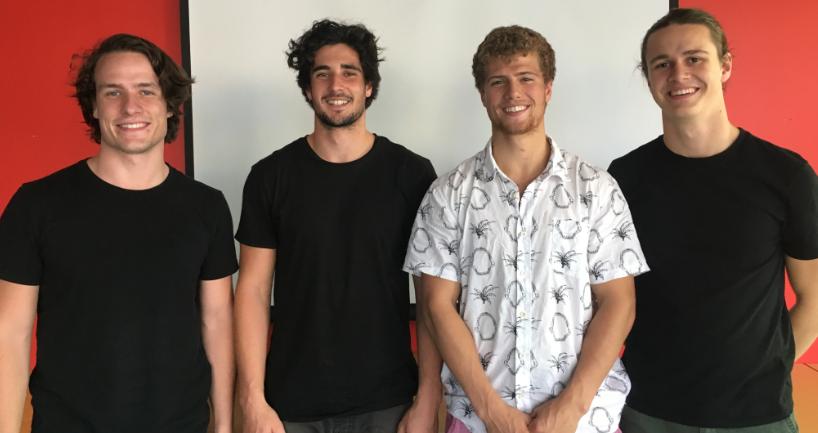
\includegraphics[width=0.85\textwidth]{img/general/boys.PNG}\\[0.25cm]

% 	SPONSOR SECTION
\large \emph{Sponsor:} Dr. Eric Lanteigne

\vfill
\end{titlepage}


\frontmatter

%---------------------------------------------------------------------
%	ABSTRACT
%---------------------------------------------------------------------
\chapter*{Abstract}
Volume 1 of the Capstone Report contains the main body of the report, including all design and analysis information. Volume 2 contains all appendices.\\

The aim of this design was to create a system for control of an unmanned airship. It was achieved by using a gondola as a ballast to move the centre of mass in relation to the centre of volume and initiate pitch changes. The design features stationary thrusters located in the XY plane of the airship, attached by carbon fibre arms which are secured to a carbon fibre keel. The keel acts as a rail for the gondola to move back and forth on. The gondola contains control equipment used to communicate with the thruster assembly wirelessly, as well as drive the gondola to the desired position. Passive breaking is achieved through the use of a linear actuator that can generate a holding force without constant power supply. Vectoring of the propellers is achieved by a servo motor mounted to a plate which connects to the thruster arms.\\

The dimensions of the airship may vary as it is not manufactured yet, and input parameters are selected by the user, meaning that the whole airship must be scalable, and its design be feasible. A GUI is implemented in MATLAB to ensure that the user selects values which are feasible and produces SolidWorks models that can be used as reference for manufacturing and design.\\

\begin{figure}[H]
	\centering
	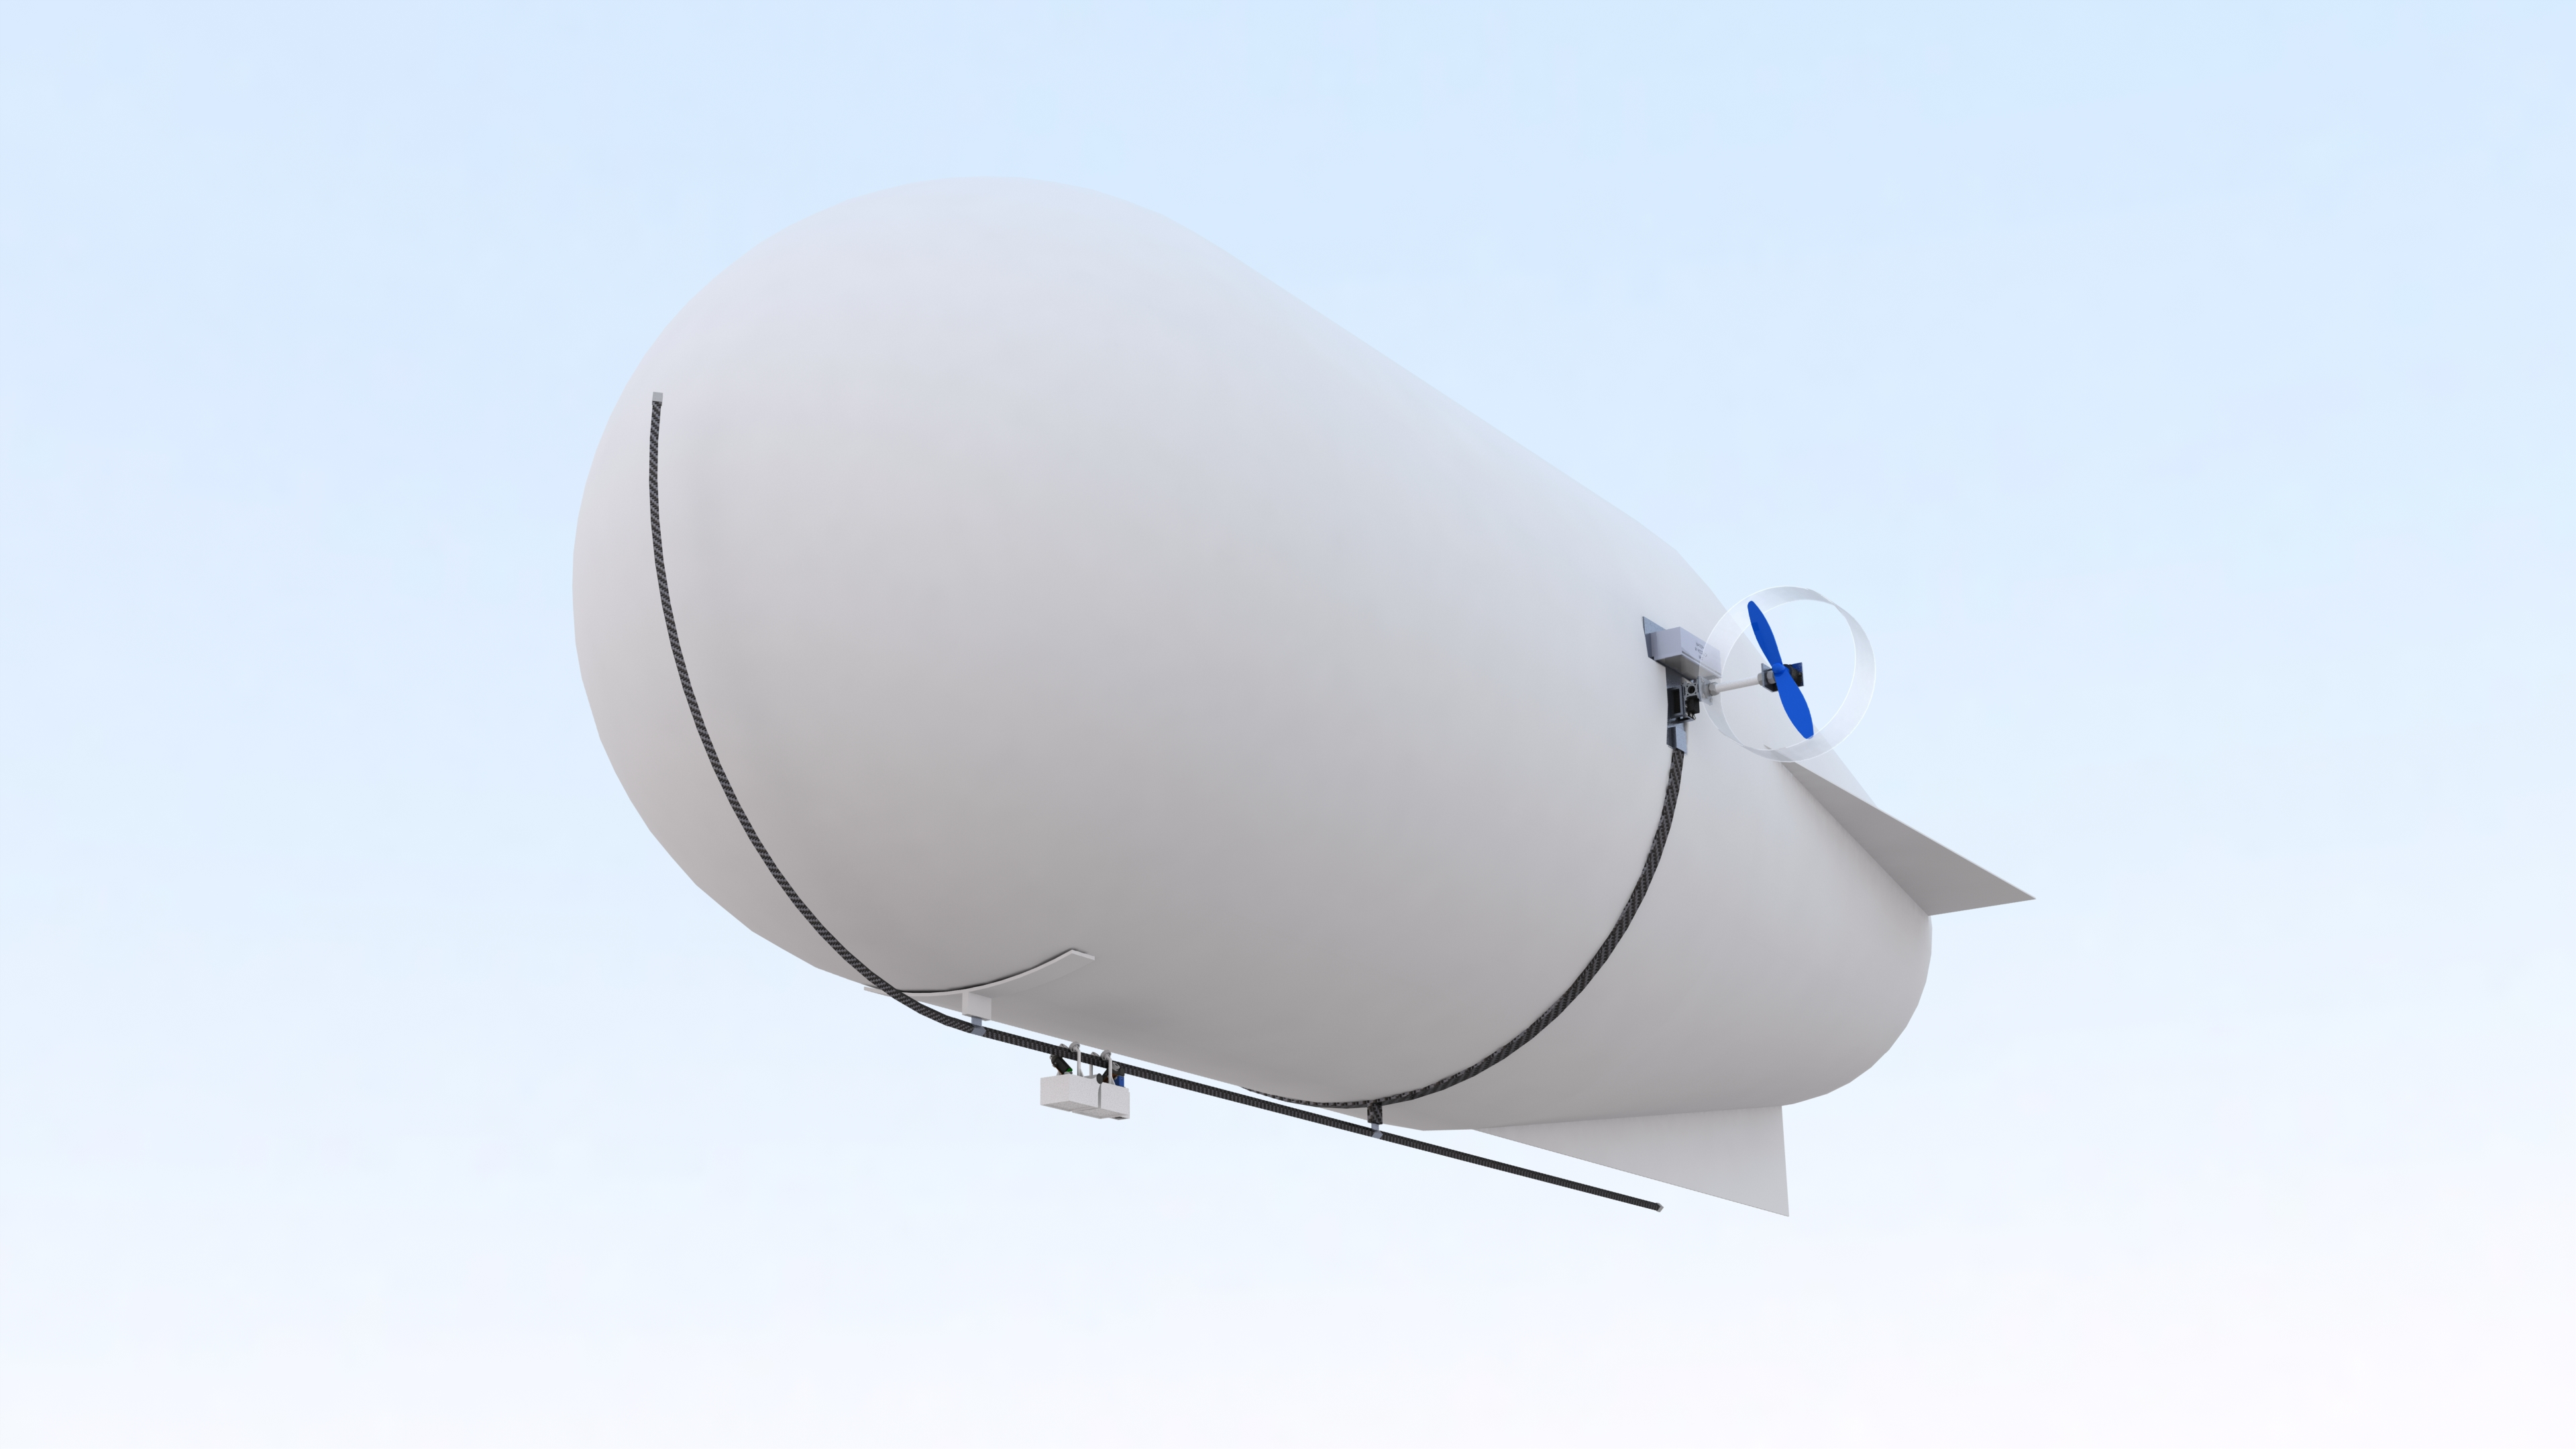
\includegraphics[width=.85\linewidth]{img/general/fullPerspective.JPG}
\end{figure}

\pagebreak

%---------------------------------------------------------------------
%	TABLE OF CONTENTS
%---------------------------------------------------------------------
\tableofcontents

%---------------------------------------------------------------------
%	LIST OF FIGURES
%---------------------------------------------------------------------
\listoffigures
\pagebreak

%---------------------------------------------------------------------
%	LIST OF TABLES
%---------------------------------------------------------------------
\listoftables
\pagebreak

%#####################################################################
%	NOMENCLATURE
%#####################################################################
\cleardoublepage  
\renewcommand{\nomname}{Nomenclature}
\markboth{\MakeUppercase\nomname}{\MakeUppercase\nomname}  
\printnomenclature
  
  \nomenclature[]{$E_p$}{Modulus of elasticity of considered plastic hub or boss [$N/mm^2$]}
  \nomenclature[]{$\sigma_s$}{Allowable design stress for plastic, $N/mm^2$}
  \nomenclature[]{$\sigma_a$}{Hoop stress, [$N/mm^2$]}
  \nomenclature[]{$i_a$}{Allowable interference, [$mm$]}
  \nomenclature[]{$d_s$}{Shaft diameter, [$mm$]}
  \nomenclature[]{$d_s$}{Shaft diameter, [$mm$]}
  \nomenclature[]{$d_i$}{Interference diameter, [$mm$]}
  \nomenclature[]{$d_o$}{Hub outer diameter, [$mm$]}
  \nomenclature[]{$F_{spring}$}{Force applied by hinge spring, [$N$]}  
  \nomenclature[]{$T_w$}{Friction wheel motor torque, [$Nm$]}
  \nomenclature[]{$F_{nfric}$}{Normal force acting on friction wheel, [$N$]}  
  \nomenclature[]{$F_{ffric}$}{Friction force acting on friction wheel, [$N$]}
  \nomenclature[]{$F_g$}{Force of gravity, [$N$]}
  \nomenclature[]{$T_{spring}$}{Torque of hinge spring, [$Nm$]}
  \nomenclature[]{$L_s$}{Length from fastener to fastener of gondola motor to hinge, [$m$]} 
  \nomenclature[]{$L_{hs}$}{Distance from the pivot of the hinge to the gondola motor fastener, [$m$]}
  \nomenclature[]{$L_{hw}$}{Distance from the gondola motor fastener to the contact point of the friction wheel, [$m$]}
  \nomenclature[]{$\mu$}{Coefficient of friction}
  \nomenclature[]{$r_{fw}$}{Radius of friction wheel, [$m$]}  
  \nomenclature[]{$L_{rx}$}{Friction wheel motors shaft length, [$m$]}
  \nomenclature[]{$a_{airship}$}{Acceleration of airship, [$m/s$]}  
  \nomenclature[]{$m_{airship}$}{Mass of airship, [$kg$]}
  \nomenclature[]{$a_{gondola1}$}{Acceleration of Gondola 1 , [$m/s^2$]}
  \nomenclature[]{$a_{gondola2}$}{Acceleration of Gondola 2 , [$m/s^2$]}
  \nomenclature[]{$m_{gondola1}$}{Mass of Gondola 1, [$kg$]}
  \nomenclature[]{$m_{gondola2}$}{Mass of Gondola 2, [$kg$]}
  \nomenclature[]{$F_{s1}$}{Force on friction wheel motor fastener 1 , [$N$]}
  \nomenclature[]{$F_{s2}$}{Force on friction wheel motor fastener 2 , [$N$]}
  \nomenclature[]{$F_{a}$}{Force on fastener a (hinge to gondola), [$N$]}
  \nomenclature[]{$F_{b}$}{Force on fastener b (hinge to gondola), [$N$]}
  \nomenclature[]{$F_{\alpha}$}{Force on fastener $\alpha$ (hinge to gondola), [$N$]}
  \nomenclature[]{$F_{\beta}$}{Force on fastener $\beta$ (hinge to gondola), [$N$]}
  \nomenclature[]{$L_a$}{Length from pivot point of hinge to fastener a , [$m$]}
  \nomenclature[]{$L_b$}{Length from pivot point of hinge to fastener b , [$m$]}
  \nomenclature[]{$L_{contact}$}{Length from contact to contact of bearings on keel, [$m$]}
  \nomenclature[]{$F_{NB}$}{Normal force applied to bearing, [$N$]}
  \nomenclature[]{$L_G$}{Width of gondola, [$m$]}
  \nomenclature[]{$L_{bc}$}{Length from centerline of gondola to fastener b, [$m$]}
  \nomenclature[]{$L_{ac}$}{Length from centerline of gondola to fastener a, [$m$]}
  \nomenclature[]{$R$}{Reaction force, [$N$]}
  \nomenclature[]{$L_{drive}$}{Length of gondola hinge to friction wheel contact, [$m$]}
  \nomenclature[]{$L_{cm}$}{Length from gondola wall to center of mass of gondola, [$m$]}
  \nomenclature[]{$L_m$}{Length from side of gondola to gondola drive motor hinge, [$m$]}
  \nomenclature[]{$H_{keel}$}{Height of the bearing arm contact point on the keel, [$m$]}
  \nomenclature[]{$F_{LA}$}{Linear actuator force, [$N$]}
  \nomenclature[]{$F_{brake}$}{Normal braking force keel reaction, [$N$]}
  \nomenclature[]{$W_{LA}$}{Weight of linear actuator, [$N$]}
  \nomenclature[]{$F_{GR}$}{Reaction force of gondola, [$N$]}
  \nomenclature[]{$F_T$}{Thruster force, [$N$]}
  \nomenclature[]{$W_T$}{Weight of thruster, [$N$]}
  \nomenclature[]{$W_A$}{Weight of thruster assembly arm, [$N$]}
  \nomenclature[]{$W_E$}{Weight of thruster enclosure, [$N$]}
  \nomenclature[]{$F_R$}{Keel to assembly arm connector reaction, [$N$]}
  \nomenclature[]{$M_R$}{Connector moment reaction, [$Nm$]}
  \nomenclature[]{$W_c$}{Weight of connection piece, [$N$]}
  \nomenclature[]{$F_{K1}$}{Keel reaction force 1, [$N$]}
  \nomenclature[]{$F_{K2}$}{Keel reaction force 2, [$N$]}
  \nomenclature[]{$F_{c1}$}{Connector moment couple force 1, [$N$]}
  \nomenclature[]{$F_{c2}$}{Connector moment couple force 2, [$N$]}
  \nomenclature[]{$c$}{Distance from neutral axis to stress location, [$m$]}
  \nomenclature[]{$w_{army}$}{Width of the bearing arm in the y direction, [$m$]}
  \nomenclature[]{$w_{armx}$}{Width of the bearing arm in the x direction, [$m$]}
  \nomenclature[]{$F_{bolt}$}{Bolt pretension force, [$N$]}
  \nomenclature[]{$\sigma _{washer}$}{Compressive force of washer, [$Pa$]}
  \nomenclature[]{$\sigma _{x}$}{Principle stress, [$Pa$]}  
  \nomenclature[]{$\sigma '$}{Von Mises Stress, [$Pa$]}
  \nomenclature[]{$S_{compressive}$}{Compressive strength of gondola material, [$Pa$]}
  \nomenclature[]{$\eta$}{Safety Factor}
  \nomenclature[]{$L_{SF}$}{Length to snap fit bearing, [$m$]}
  \nomenclature[]{$M_1$}{Reaction moment on bearing arm, [$Nm$]}
  \nomenclature[]{$F_{RSF}$}{Force of snap fit bearing [$N$]}
    
%---------------------------------------------------------------------
%	MAIN BODY
%---------------------------------------------------------------------
\pagestyle{fancy}
\setlength{\headheight}{14.5pt} 
\fancyhf{}
\rhead{\rightmark}
\cfoot{\thepage}

\mainmatter

%#####################################################################
%	INTRODUCTION
%#####################################################################
\subfile{./tex/chapter1Introduction.tex}

%#####################################################################
%	PROPOSED DESIGN
%#####################################################################
\subfile{./tex/chapter2ProposedDesign.tex}

%#####################################################################
%	ANALYSIS
%#####################################################################
\chapter{Analysis}
\subfile{./tex/analysisIntro.tex}
\subfile{./tex/analysisHighLevelParametrization.tex}

\section{System Modelling} \label{modelling}
\subfile{./tex/analysisSystemModelling.tex}
\subfile{./tex/analysisDragAnalysis.tex}
\subfile{./tex/analysisEnvelope.tex}

\section{Component Analysis}
\subfile{./tex/analysisThrusterAssemblySelection.tex}
\subfile{./tex/analysisThrusterShaft.tex}
\subfile{./tex/analysisThrusterArms.tex}
\subfile{./tex/analysisConnector.tex}
\subfile{./tex/analysisFrictionWheelSlip.tex}
\subfile{./tex/analysisHingeBolts.tex}
\subfile{./tex/appendixLinearActuator.tex}
\subfile{./tex/analysisGondolaArm.tex}
\subfile{./tex/analysisSnapFit.tex}

%#####################################################################
%	DISCUSSION & CRITICAL REVIEW
%#####################################################################
\subfile{./tex/chapter4Discussion.tex}

%#####################################################################
%	BIBLIOGRAPHY
%#####################################################################
\bibliographystyle{plainnat}
\bibliography{library}

\pagebreak

%#####################################################################
%	APPENDICES
%#####################################################################
\appendix
%-----------------------------------------------------------------
%	GUI INSTRUCTIONS HERE
%-----------------------------------------------------------------
\subfile{./tex/appendixGUI.tex}

%-----------------------------------------------------------------
%	MATLAB CODE HERE
%-----------------------------------------------------------------
\chapter{Code}
\section{Main} \label{code:main}
\lstinputlisting[language=Octave]{MATLAB/dummy.m} %USE THIS FORMAT TO INSERT CODE
\section{Design Code} \label{code:designCode}
\subsection{Envelope Size} \label{code:envelope}
\subsection{Propeller and Motor Selection} \label{code:motorSelect}
\subsection{Battery Selection} \label{code:batterySelect}
\subsection{Battery, Motor, and Propeller Data} \label{code:bmpData}
\subsection{Thruster Shaft Analysis} \label{code:thrusterShaft}
\subsection{Thruster Arm Analysis} \label{code:arm}
\subsection{Airship Mass} \label{code:mass}
\subsection{Gondola Forces} \label{code:gondolaforce}
\subsection{Gondola Analysis} \label{code:gondola}
\subsection{Pitch Plot} \label{code:pitch}

\section{Generic}
\subsection{Cauchy} \label{code:cauchy}
\subsection{Force Solver} \label{code:forceSolver}
\subsection{Centre Mass} \label{code:CM}
\subsection{Gondola Force Rotator} \label{code:rotate}

%-----------------------------------------------------------------
%	ADDITIONAL MATERIAL HERE
%-----------------------------------------------------------------
\chapter{Additional Material}
\subfile{./tex/analysisGondolaArmDeflection.tex}
\subfile{./tex/analysisArmFatigue.tex}
\subfile{./tex/analysisThrusterAdhesion.tex}
\subfile{./tex/analysisMotorShaft.tex}
\subfile{./tex/appendixNylonShaftScrew.tex}
\subfile{./tex/appendixVectoringMotor.tex}
\subfile{./tex/appendixGondolaHinge.tex}
\subfile{./tex/appendixBearings.tex}
\subfile{./tex/appendixForceSolver.tex}
\subfile{./tex/appendixCauchy.tex}
\subfile{./tex/appendixThrustCalculations.tex}
\subfile{./tex/appendixDragAnalysis.tex}

%-----------------------------------------------------------------
%	DATA SHEETS HERE
%-----------------------------------------------------------------
\subfile{./tex/appendixDataSheets.tex}

%-----------------------------------------------------------------
%	ENGINEERING DRAWINGS HERE
%-----------------------------------------------------------------
\subfile{./tex/appendixDrawings.tex}

%-----------------------------------------------------------------
%	MEETING MINUTES
%-----------------------------------------------------------------
\begin{landscape}
\subfile{./tex/appendixMinutes.tex}
\end{landscape}
%-----------------------------------------------------------------
%	RECOMMENDATIONS FOR IMPROVING THE COURSE
%-----------------------------------------------------------------
\chapter{Recommendations for Improving the Course}
lol

\end{document}